\newpage
\null
\thispagestyle{empty}
\newpage
\pagestyle{plain}
\pagenumbering{roman}
%\renewcommand{\thepage}{\Alph{page}}

\section{Plán práce a jeho plnenie}

Plán práce:

\begin{itemize}
	\item DP1:
		\begin{itemize}
			\item analýza problematiky
			\item prvotné experimenty
		\end{itemize}
	\item DP2:
		\begin{itemize}
			\item vybratie vhodného datasetu
			\item experimentovanie s modelmi pozornosti zdola nahor
			\item nájdenie najlepšieho modelu pre ďalšie experimentovanie
		\end{itemize}
	\item DP3:
		\begin{itemize}
			\item experimentovanie so semantickým kontextom a faktormi pozornosti zhora nadol
			\item výber najlepšieho modelu
			\item testovanie a porovnanie s existujúcimi riešeniami
		\end{itemize}
\end{itemize}

Moje vyjadrenie k plánu práce považujem za irelevantné, rovnako ako samotný plán, nakoľko sa neustále menil a nemalo zmysel ho v jednotlivých semestroch určovať. K riešeniu projektu sme pristúpili agilne, pružne sme reagovali na zmeny a výsledky z jednotlivých experimentov, podľa ktorých sme počas celej práce upravovali jej smerovanie. 

\newpage
\section{Obsah priloženého elektronického nosiča}

Štruktúra dát na elektronickom nosiči:

\begin{itemize}
	\item \textbf{datasets} - datasety použité na trénovanie a testovanie, vzorka upraveného pripraveného datasetu pre neurónovú sieť
	\item \textbf{source\_codes} - zdrojové kódy
	\item  \textbf{models} - uložené natrénované modely
	\item \textbf{document} - pdf verzia odovzdávanej práce
\end{itemize}

\newpage
\section{Technická dokumentácia}
\label{technical_doc}

Celé popisované riešenie bolo vyvinuté a otestované na Linux-ových operačných systémoch Ubuntu 18.04.2 LTS a Fedora 28 - na nich vieme  zaručiť správne korektné fungovanie priložených skriptov. Tie sú napísané v jazyku Python vo verzie 3.5, za použitia nasledovných knižníc:

\begin{itemize}
	\item TensorFlow - vo verzii 1.13.1, knižnica pre prácu s neurónovými sieťami 
	\item Keras - vo verzii 2.2.2, vysoko úrovňová knižnica pre prácu s neurónovými sieťami, v našom riešení využíva nižšie úrovňový TensorFlow (za použitia napríklad knižnice Theano skripty nebudú fungovať)
	\item Matplotlib - verzia 3.0.0, knižnica pre 2D vykreslovanie a prácu z obrázkami, použitá pri vizualizáciách predikcií
	\item OpenCV - verzia 3.4.4.19, knižnica pre počítačové videnie a strojové učenie, použitá pre prácu s obrázkami
	\item SciPy\footnote{https://docs.scipy.org/doc/scipy/reference/index.html} - verzia 1.1.0, knižnica pre prácu s dátami
	\item NumPy\footnote{https://www.numpy.org/} - verzia 1.15.2, knižnica pre prácu s dátami
	\item Image Processing SciKit (scikit-image)\footnote{https://scikit-image.org/} - verzia 0.14.1, knižnica pre jednoduché spracovanie obrázkov
\end{itemize}

Verzie knižníc uvádzame z dôvodu kompatibility riešenia, napríklad je možné, že skripty budú fungovať aj na iných verziách knižníc pre práce s neurónovými sieťami (Keras, TensorFlow), ale v iných verziách nemusia byť schopné načítať uložené modely. 

Čo sa týka hardvérového vybavenia, celé riešenie bolo natrénované na grafickej karte Nvidia GeForce GTX 1080 Ti s veľkosťou 12gb a RAM s veľkosťou 32gb. Trénovanie aj predikcie je možné uskutočnovať aj na CPU, bude to však mať značné dopady na výkon. Trénovanie je možné aj na menšej grafickej karte, je však nutné zmenšiť aj veľkosť dávky (z angl. batch size) pre jedno trénovanie.

\section{Používateľská príručka}

%TODO vyriesit cislovanie
\newpage
\pagenumbering{gobble}
\section{Podrobný diagram architektúry s kombináciou VGG16 a autoenkóderu}
\label{vgg16_autoencoder_architecture_detailed}
\begin{figure}[H]
	\begin{center}
		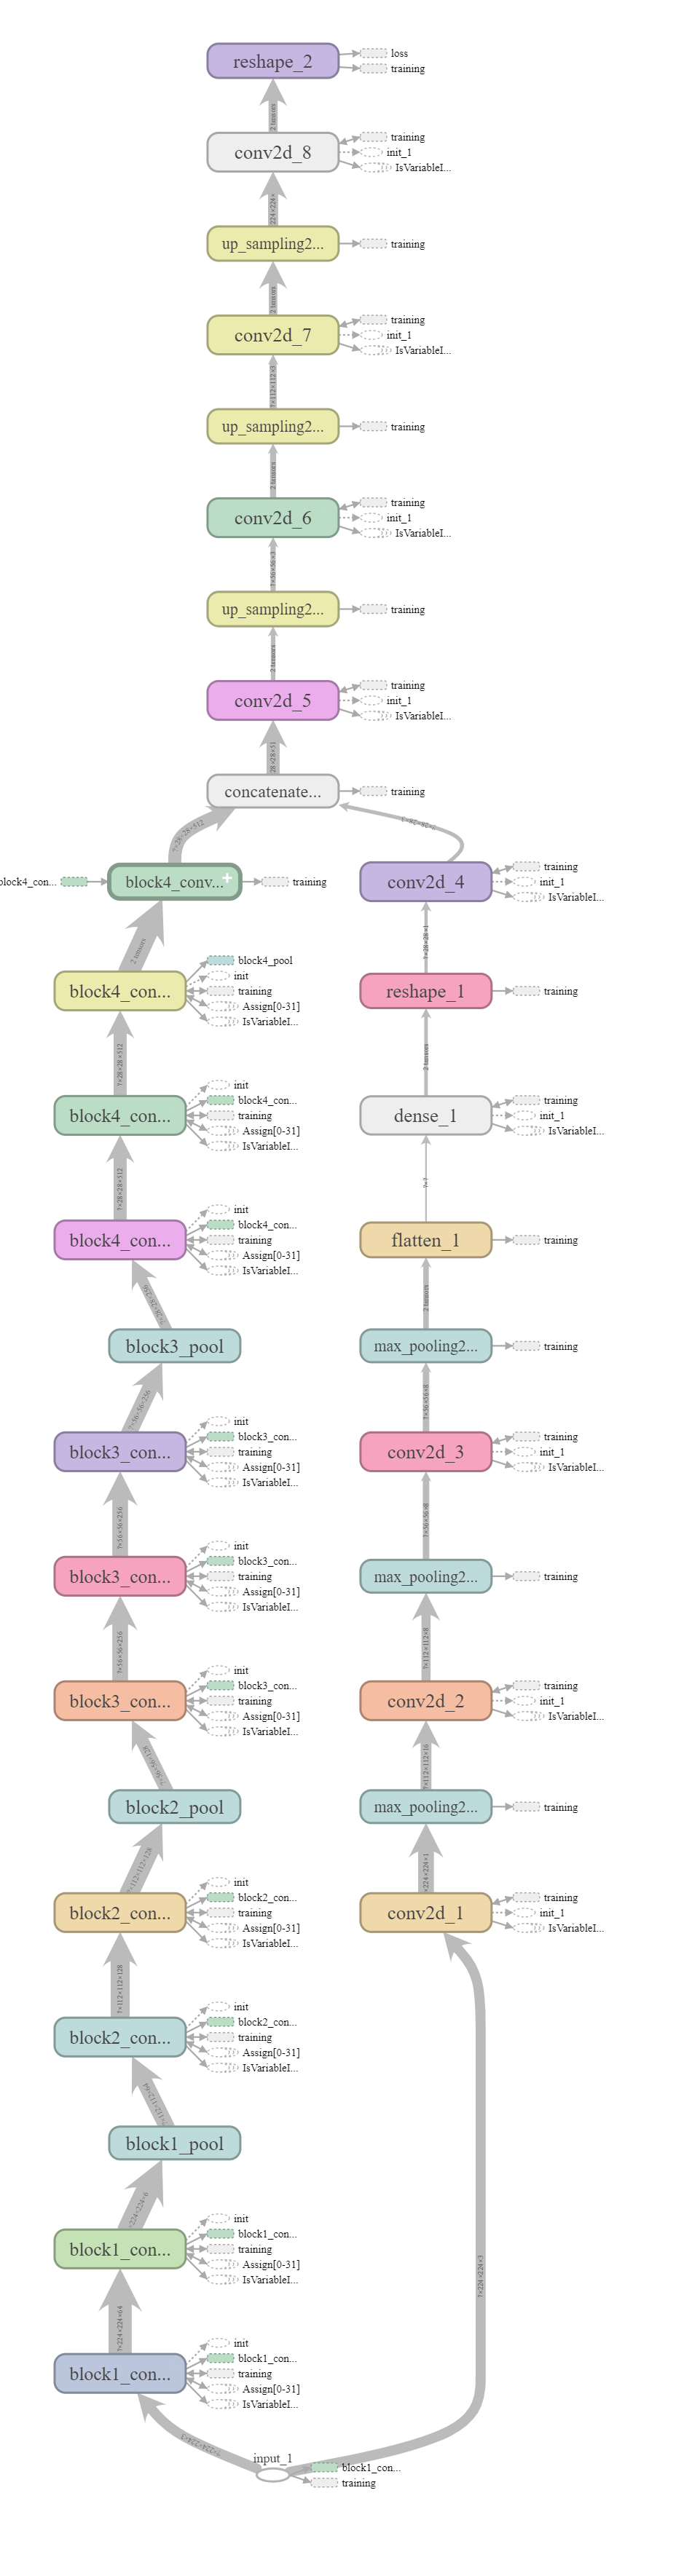
\includegraphics[scale=0.24]{vgg16_with_autoencoder_full.png}
		\caption[Podrobný diagram architektúry VGG16 s autoenkóderom]{Podrobný diagram architektúry VGG16 s autoenkóderom}
	\end{center}
\end{figure}

%TODO Technicka dokumentacia? prostredie, hardver, kniznice, atd.

%TODO pouzivatelska prirucka

